% arara: pdflatex
% arara: pdflatex
% arara: pdflatex

% options:
% thesis=B bachelor's thesis
% thesis=M master's thesis
% czech thesis in Czech language
% slovak thesis in Slovak language
% english thesis in English language
% hidelinks remove colour boxes around hyperlinks

\documentclass[thesis=B,czech]{FITthesis2}[2012/06/26]

\usepackage[utf8]{inputenc} % LaTeX source encoded as UTF-8

\usepackage{graphicx} %graphics files inclusion
% \usepackage{amsmath} %advanced maths
% \usepackage{amssymb} %additional math symbols

\usepackage{dirtree} %directory tree visualisation

\usepackage[shortlabels]{enumitem}

% % list of acronyms
% \usepackage[acronym,nonumberlist,toc,numberedsection=autolabel]{glossaries}
% \iflanguage{czech}{\renewcommand*{\acronymname}{Seznam pou{\v z}it{\' y}ch zkratek}}{}
% \makeglossaries

\newcommand{\tg}{\mathop{\mathrm{tg}}} %cesky tangens
\newcommand{\cotg}{\mathop{\mathrm{cotg}}} %cesky cotangens

% % % % % % % % % % % % % % % % % % % % % % % % % % % % % % 
% ODTUD DAL VSE ZMENTE
% % % % % % % % % % % % % % % % % % % % % % % % % % % % % % 

\department{Obor Webové a softwarové inženýrství (BI-WSI), zaměření Softwarové inženýrství\\Katedra softwarového inženýrství}
\title{Webová aplikace pro online web scraping}
\authorGN{Jakub} %(křestní) jméno (jména) autora
\authorFN{Drahoš} %příjmení autora
\authorWithDegrees{Jakub Drahoš} %jméno autora včetně současných akademických titulů
\author{Jakub Drahoš} %jméno autora bez akademických titulů
\supervisor{Martin Podloucký}
\keywordsCS{web scraping, extrakce dat, aplikace, JavaScript, rozšíření do Chromu, právní rozbor}
\keywordsEN{web scraping, data extraction, application, JavaScript, Chrome extension, legal analysis}

\begin{document}
	
	% \newacronym{CVUT}{{\v C}VUT}{{\v C}esk{\' e} vysok{\' e} u{\v c}en{\' i} technick{\' e} v Praze}
	% \newacronym{FIT}{FIT}{Fakulta informa{\v c}n{\' i}ch technologi{\' i}}
	
	\begin{introduction}
		\paragraph*{Klíčová slova} \thekeywordscs{}
		\paragraph*{Keywords} \thekeywordsen{}
		
		\section*{Cíle práce}
		Hlavním cílem této práce je návrh a tvorba webové aplikace, která bude umožňovat uživatelům extrahovat požadovaná data z~libovolné stránky v~reálném čase bez jakékoli nutné znalosti programování. Při specifikaci požadavků tohoto softwaru se přihlídne k analýze stávajících řešení, jež je vedlejším cílem této práce. Druhým vedlejším cílem je poskytnout čtenáři úvod do právní problematiky web scrapingu a shrnout na jednom místě fakta, která máme k dispozici.
		
		Neméně důležitou součást práce tvoří dodržení klasického vývojového cyklu softwarového projektu -- analýza, design, implementace a testování.
		
		Klíčovým aspektem aplikace je též \emph{přehlednost a jednoduchost uživatelského rozhraní} -- důraz bude kladen na intuitivní a rychlé ovládání.
		
		Naopak v rozsahu této práce není tvorba web crawlera ani žádného jiného podobného mechanismu, jenž by systematicky a především \emph{automatizovaně} procházel danou oblast webu.
		
		\section*{Motivace}
		Téma web scrapingu je v dnešní době velice aktuální a čím více dat produkujeme, tím více bude stoupat potřeba tyto informace určitým způsobem získávat a zpracovávat. Téměř kdokoli, kdo pracuje s daty dostupnými z internetu, bude nucen využít nějaký nástroj k vytěžování, aby byl vůbec schopný udržet krok s konkurencí.
		
		Tedy důvod k vytvoření softwaru umožňující extrahovat data z webových stránek je jasný. Ač podobných nástrojů existuje několik, jejich obsluha je poměrně složitá a je nutné strávit určitý čas, než se člověk seznámí s jejich fungováním a může je naplno využít. Právě tento aspekt se snaží aplikace vyvíjená v rámci této bakalářské práce eliminovat -- motivací je tak poskytnout uživatelům možnost jednoduše a rychle vytěžit požadovaná data bez zbytečného zdržování a dlouhého času stráveného seznamováním se s nástrojem.
		
		Jak již bylo řečeno, přínos aplikace spočívá především v její jednoduchosti. Z toho mohou těžit hlavně uživatelé, kteří se nezabývají programováním nebo tvorbou webových stránek. Využije ji tak kdokoli, kdo potřebuje jednorázově získat data z libovolné internetové stránky, která obsahuje velké množství dat pohromadě na jedno místě. Z důvodu prozatím chybějícího crawlingu (automatizovaného procházení) je naopak nevhodná k pravidelnému získávání dat (jako je například dlouhodobé sledování cen produktů) či ke zpracování stránek, kdy se jednotlivá data nacházejí rozptýlená po celé doméně.
		
		To, čím je tato práce unikátní, je ale rozbor právního aspektu web scrapingu. V žádném případě se nejedná o hlubokou analýzu, která by byla očekávána od studenta právnické fakulty. Zároveň ale shrnuje podstatné poznatky a fakta z dané oblasti na jednom místě. Při hledání tohoto tématu na internetu totiž uživatel narazí na jeden nešvar -- téměř vše začíná odstavcem ve stylu \uv{...nejsem právník a toto je jen můj názor...}, informace jsou velmi kusé a chybí jim nějaká ucelená struktura. Tento neduh se práce snaží napravit a představuje tak vstupní bránu do této rozsáhlé problematiky. Zároveň může pomoct všem vývojářům, kteří tvoří software určený k web scrapingu.
		
		\section*{Členění práce}
		Kapitola 1 je věnována analýze tématiky web scrapingu. První sekce shrnuje obecné informace, následuje pohled z právní strany věci a nakonec analýza stávajících řešení problému. Kapitola 2 se zaměřuje na návrh aplikace -- specifikace požadavků, architektura systému, návrh uživatelského rozhraní. Ve třetí kapitole je popsána realizace daného návrhu, výběr použitých technologií a odůvodnění rozhodnutí, která byla učiněna. Poslední kapitola je věnovaná testování celé aplikace.
	\end{introduction}
	
	
	% ================================================================================================
	
	
	\chapter{Analýza}
	
	\section{Analýza konkurenčních nástrojů}
	První skupinou, na kterou můžeme při hledání na internetu narazit, jsou společnosti, které nabízejí zákazníkům kompletní péči v~rámci extrakce dat. Cílí především na velké korporace, jimž postaví scrapovací nástroj přesně na míru, který poté také hostují a spravují. Zákazník tedy dostane data a o~nic víc se již nemusí starat. Jako příklad lze jmenovat třeba ContentGrabber, Mozenda a další.
	
	Pro tuto práci mnohem relevantnější kategorií je konkurenční nabídka nástrojů poskytujících uživatelům rozhraní k~web scrapingu. Zaměříme se pouze na takové nástroje, které nevyžadují jakoukoli znalost programování -- tedy žádné knihovny, API a nástroje pro budování vlastních scraperů.
	
	Mezi ty největší představitele patří ParseHub, Octoparse, WebScraper, Data Scraper a Dexi.io. Čtyři ze zmíněných nástrojů jsou volně dostupné (které mají však velmi omezenou funkcionalitu a pokročilejší operace se odemknou až s~určitým platebním plánem -- tzv. freemium model) a jeden poskytuje bezplatně pouze 7denní zkušební verzi.
	
	Předtím, než bude možné jednotlivé nástroje porovnávat, je nutné určit kritéria, podle kterých lze hodnotit kvalitu daného nástroje. Především půjde o~jednoduchost používání, celkovou přehlednost a rychlost, se kterou se uživatel dostane k~požadovaným datům. Důležitý je také způsob výběru dat, možnosti exportu získaných dat, jak aplikace sama dokáže uživatele seznámit s~používáním a také, v~jaké formě se nástroj vůbec používá a čím se od ostatních odlišuje (ať už v~pozitivním či negativním smyslu). 
	
	Poj\v{d}me se tedy na některé nástroje podívat blíže:
	
	\subsection{ParseHub}
	\textbf{Výhody:}
	\begin{itemize}
		\item výběr dat jak pomocí klikání (inteligentní hledání vzorců/podobností na základě prvních dvou kliknutí), tak pomocí XPath, regulárních výrazů nebo CSS selektorů
		\item aplikace obsahuje interaktivní tutoriál, který na jednoduchých příkladech ukáže, jak s~nástrojem zacházet
		\item možnost získání dat různými formami - přes API, jako CSV/XLS, do GoogleSheets nebo do Tableau
		\item různé módy kliknutí (výběr, relativní výběr, kliknutí), zooming in/out na HTML elementy -- když se uživatel netrefí (nebo ani trefit nemůže) přesně na požadovaný prvek, lze na něj lehce přejít pomocí této funkce
		\item automatická rotace IP adresy (tedy nedochází k~blokování ze strany serveru)
	\end{itemize}
	\textbf{Nevýhody:}
	\begin{itemize}
		\item nutnost stažení aplikace (ale je zde podpora pro Windows, Linux i Mac)
		\item aplikace je celkově těžkopádná, nemá moc přívětivé uživatelské rozhraní, ovládání působí nepřehledně a přehlceně -- na uživatele se vyvalí hodně informací a možností najednou
	\end{itemize}
	\begin{figure}[h]
		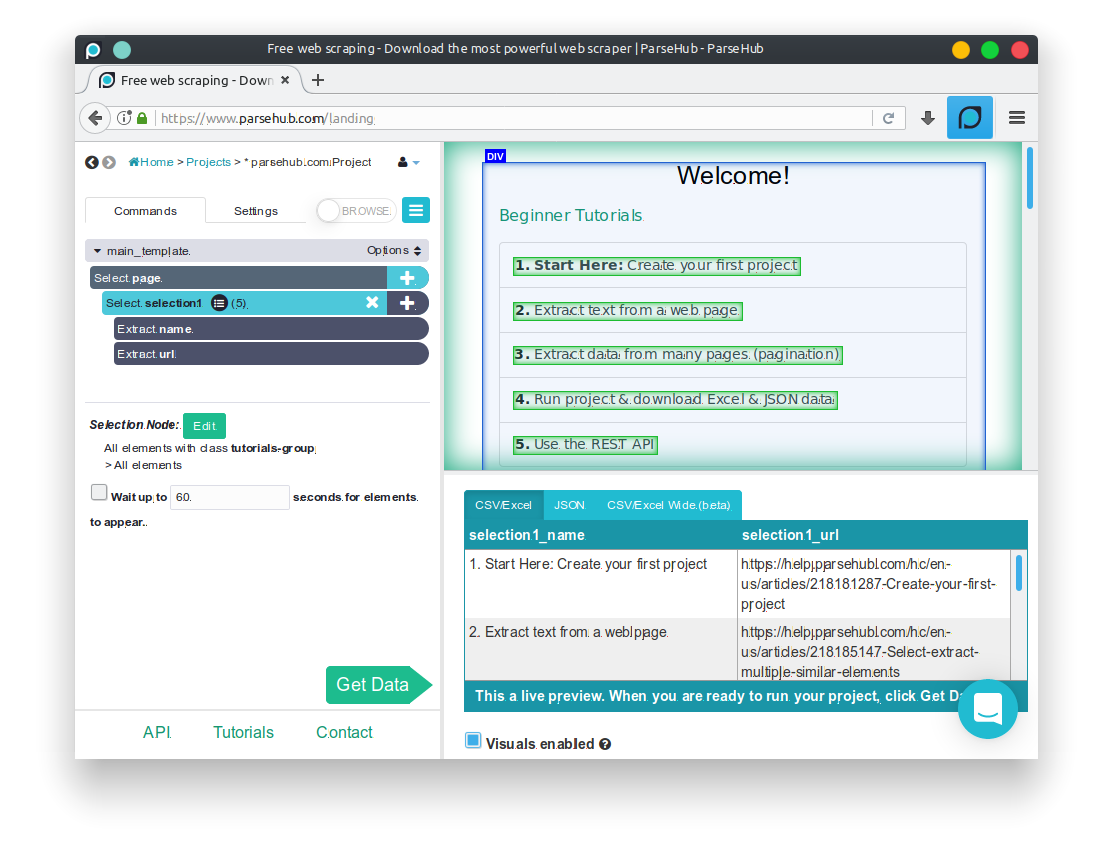
\includegraphics[width=\linewidth]{images/ParseHub.png}
		\caption{ParseHub\cite[snímek pořídil autor]{parsehub}}
		\label{fig:parseHub}
	\end{figure}
	
	
	\subsection{Octoparse}
	\textbf{Výhody:}
	\begin{itemize}
		\item výběr dat jak pomocí klikání (inteligentní hledání vzorců/podobností na základě prvních dvou kliknutí), tak pomocí XPath nebo regulárních výrazů
		\item nástroj obsahuje hotové šablony, které mohou velmi urychlit práci
		\item pestrá paleta možností (branch judgment, tvoření smyček apod.) -- dá se vytvořit téměř jakákoli logika procházení webu a extrakce dat
		\item lehký způsob, jak scrapování automatizovat
		\item možnost řídit tasky přes API (a získávat tak data taktéž přes API); data jdou nahrát rovnou i do lokální databáze
	\end{itemize}
	\textbf{Nevýhody:}
	\begin{itemize}
		\item nutnost stažení aplikace (která je navíc pouze pro Windows)
		\item těžkopádné a pomalé ovládání, neintuitivní rozhraní
		\item tutoriál je v~podstatě nic neříkající
		\item připravených šablon je jenom pár a jsou velmi konkrétní
	\end{itemize}
	\begin{figure}[h]
		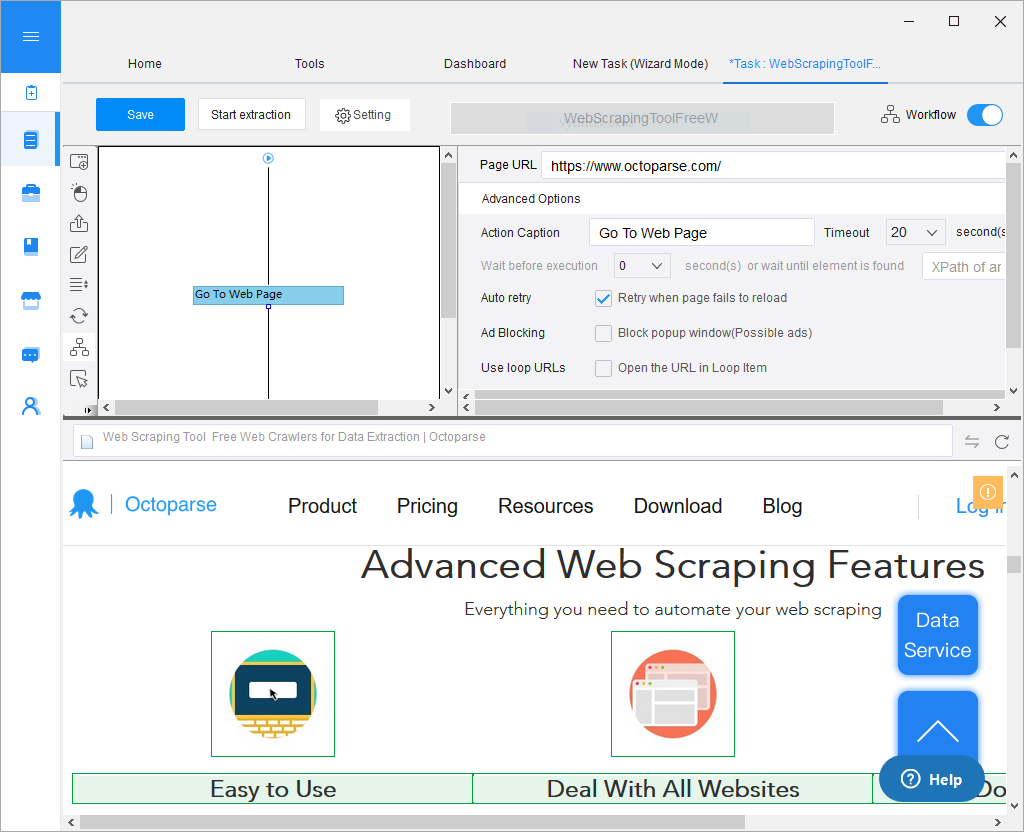
\includegraphics[width=\linewidth]{images/Octoparse.png}
		\caption{Octoparse\cite[snímek pořídil autor]{octoparse}}
		\label{fig:octoparse}
	\end{figure}
	
	
	\newpage
	\subsection{WebScaper}
	\begin{figure}
		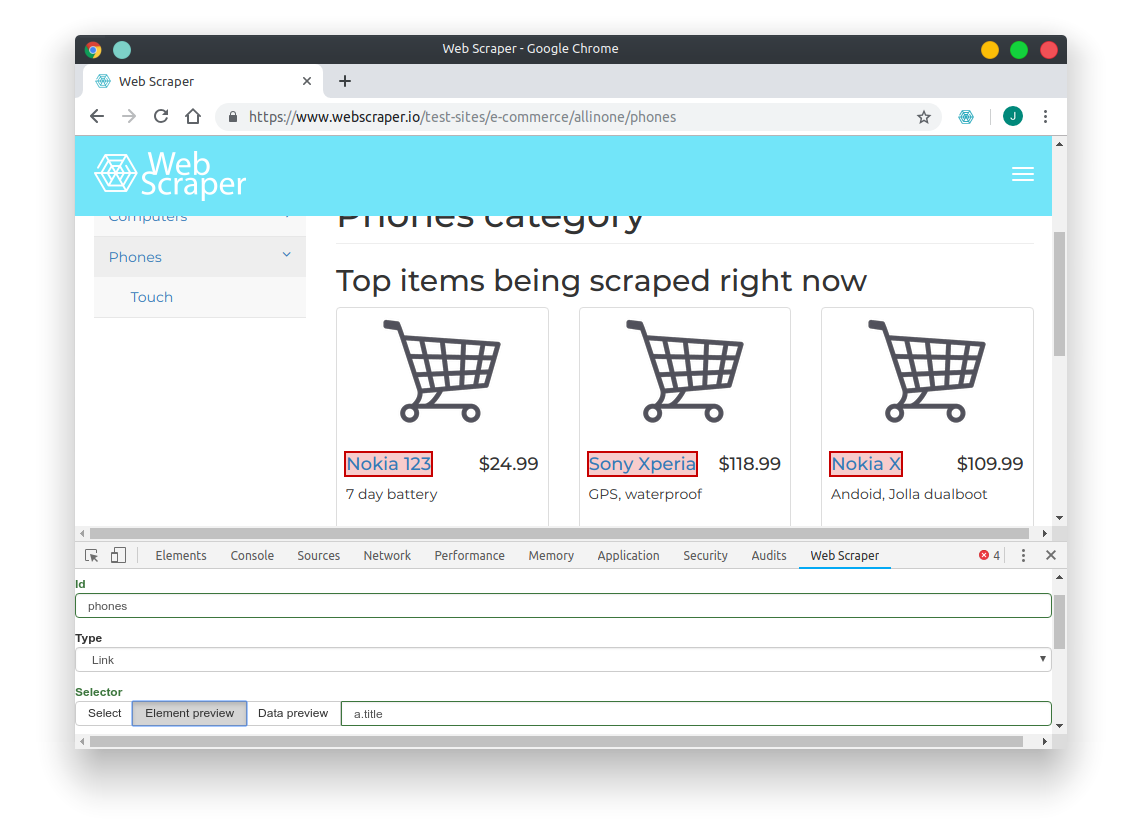
\includegraphics[width=\linewidth]{images/WebScraper.png}
		\caption{WebScraper\cite[snímek pořídil autor]{webscraper}}
		\label{fig:webScraper}
	\end{figure}
	\textbf{Výhody:}
	\begin{itemize}
		\item jednoduchá instalace (jedná se pouze o~rozšíření do prohlížeče Google Chrome); scrapování probíhá skrze vývojářskou konzoli
		\item výběr dat pomocí klikání (inteligentní hledání vzorců/podobností na základě prvních dvou kliknutí)
		\item tutoriály jsou formou videí -- jednoduché, rychlé a naprosto postačující
		\item různé typy elementů, které vybíráme (text, odkaz, scroll down), takže lze celkem snadno projít celou doménu
		\item možnost získání dat různými formami -- přes API, jako CSV/XLS nebo do Dropboxu
		\item klávesové zkratky při výběru elementů velmi usnadňují práci
		\item možnost využít jejich cloud k~automatizaci celého procesu
		\item oproti konkurenci nabízí přehledné rozhraní, rychlé a jednoduché používání
	\end{itemize}
	\textbf{Nevýhody:}
	\begin{itemize}
		\item nutnost používat Google Chrome, což pro některé uživatele může být překážka
		\item nelze vyhledávat podle klíčových slov ani podle HTML nebo CSS, tudíž všechno se musí manuálně naklikat
	\end{itemize}
	
	
	\subsection{Dexi.io}
	\begin{figure}[h]
		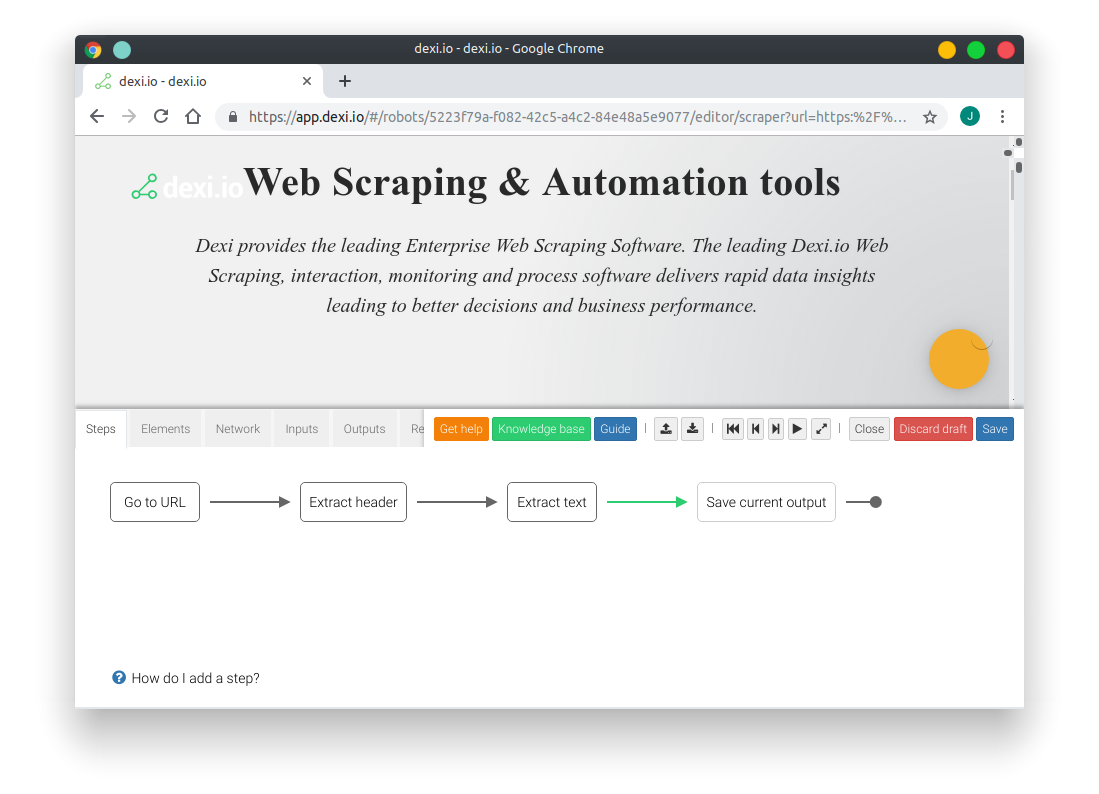
\includegraphics[width=\linewidth]{images/Dexiio.png}
		\caption{Dexi.io\cite[snímek pořídil autor]{dexio}}
		\label{fig:dexi.io}
	\end{figure}
	\textbf{Výhody:}
	\begin{itemize}
		\item bez nutnosti stahování aplikace -- vše se ovládá přes webové rozhraní
		\item výběr dat jak pomocí klikání (inteligentní hledání vzorců/podobností na základě prvních dvou kliknutí), tak pomocí HTML, CSS nebo textové shody
		\item mnoho návodů dostupných na stránkách, interaktivní rádce přímo při scrapování
		\item všechny možné druhy kliknutí, takže lze lehce projít celou doménu
		\item možnost exportovat data do CSV, JSON, XLS, získat přes API, poslat do Google Drive, Google Sheets nebo Amazon S3
		\item různé módy aplikace -- scraping, crawler, pipes (skládání menších scrape botů) a autobot (extrahování z~více stránek najednou se stejným rozložením); možnost takto automatizovat celý proces.
		\item nápomocné jsou různé addony (např. na obcházení Captchy)
	\end{itemize}
	\textbf{Nevýhody:}
	\begin{itemize}
		\item široká nabídka možností, a tak chvílí trvá, než se člověk zorientuje
		\item placený nástroj, zadarmo je dostupná pouze týdenní zkušební verze
		\item úvodní tutoriál je velmi strohý a žádné velké seznámení s~nástrojem se nekoná
	\end{itemize}
	
	
	\subsection{Data Scraper}
	\textbf{Výhody:}
	\begin{itemize}
		\item jednoduchá instalace (jedná se pouze o~rozšíření do prohlížeče Google Chrome).
		\item velmi jednoduché ovládání a přehledné rozhraní
		\item výběr dat probíhá pomocí klikání
		\item klikáním se utváří JQuery selektor, který si uživatel může podle svého upravit a doladit tak drobné detaily, jež by jinak nutně zahltily uživatelské rozhraní (tedy je možné vyhledávat i podle HTML tagů, id, CSS selektorů -- zkrátka vše, co umí klasické JQuery)
		\item různé druhy kliknutí
		\item možnost spustit na stránce libovolný JavaScriptový kód v~rámci scrapování
	\end{itemize}
	\textbf{Nevýhody:}
	\begin{itemize}
		\item nutnost používat Google Chrome, což pro některé uživatele může být překážka
		\item oproti ostatním nástrojům se může zdát velmi chudý na různé funkce
	\end{itemize}
	\begin{figure}
		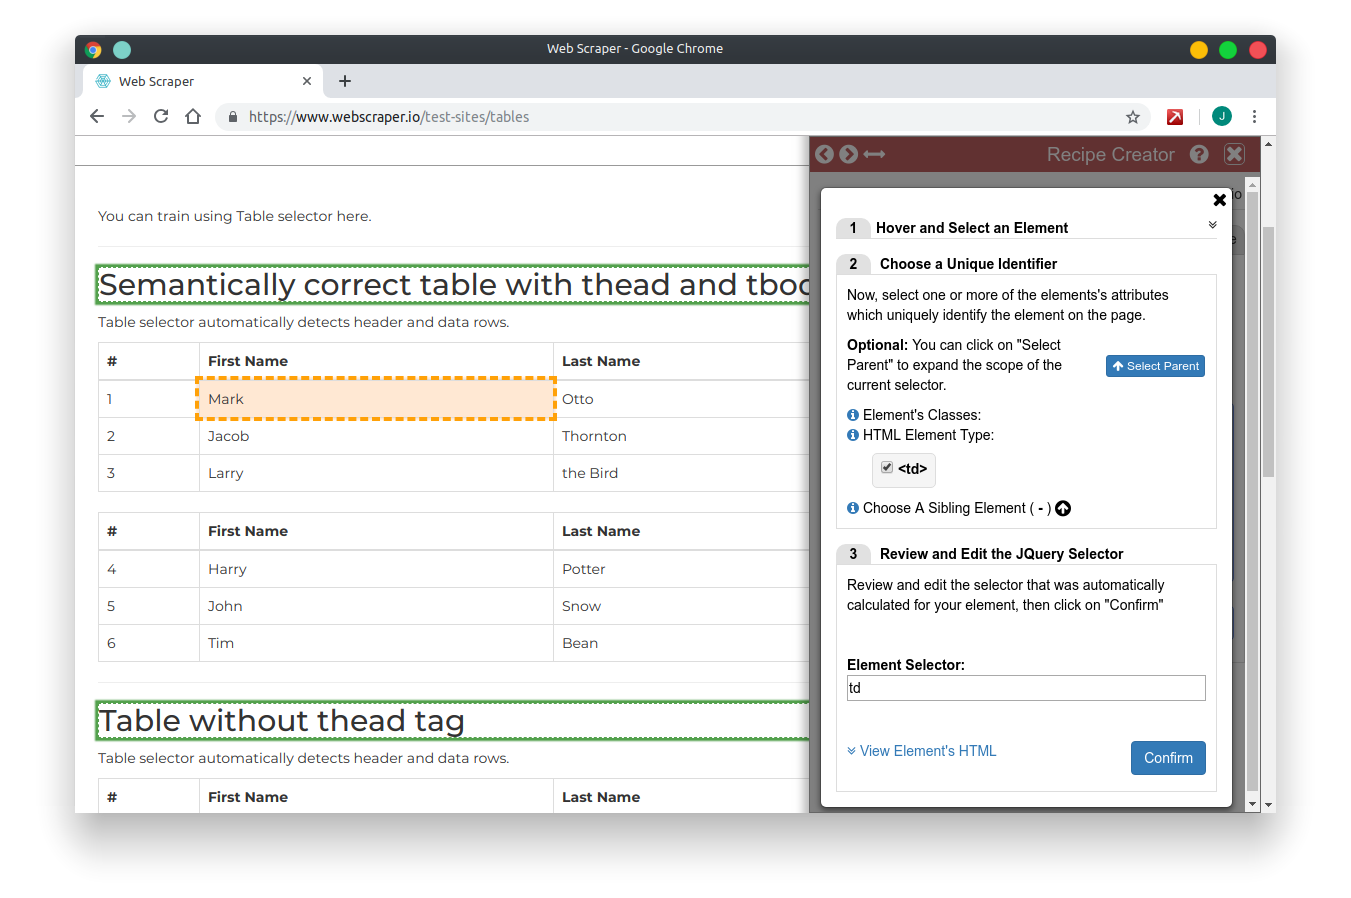
\includegraphics[width=\linewidth]{images/DataScraper.png}
		\caption{Data Scraper\cite[snímek pořídil autor]{data_scraper}}
		\label{fig:dataScraper}
	\end{figure}

	\subsection{Shrnutí}
	Jak jsme viděli, největšími neduhy, které se prolínají napříč valnou většinou aplikací, jsou \emph{těžkopádné uživatelské rozhraní}, \emph{neintuitivní ovládání} a \emph{rychlost} (nebo spíš pomalost), se kterou se uživatel dostane k~požadovaným datům. Také jsme se přesvědčili, že nejpříjemnější cestou je celou aplikaci ovládat přes webové rozhraní  \emph{bez nutnosti stahování a instalace}.
	
	Na druhou stranu se lze u~konkurence i inspirovat. Za vyzdvižení stojí určitě \emph{různé druhy výběru dat} -- \emph{klikání} přímo na stránce spolu s~inteligentním hledáním podobných prvků jistě tvoří mocný mechanismus. Avšak je potřeba zajistit i ostatní způsoby výběru (jako je např. \emph{textová shoda, HTML tagy, CSS selektory}) pro případ, kdy je pouhé klikání zdlouhavé či nevyhovující. Rovněž široký výběr způsobů exportu dat, intuitivní klávesové zkratky a zooming in/out na prvky může uživatelům zpříjemnit práci s~nástrojem.
	
	
	% ================================================================================================
	
	\chapter{Realizace}
	
	\section{Diskuze možných řešení}
	Původní záměr byl vytvořit webovou aplikaci. Důvod je jednoduchý, nikdo v dnešní době nechce cokoli stahovat a instalovat. Vzhledem k důrazu vyvíjeného nástroje kladeného na jednoduchost a rychlost používání je tak webová aplikace jasnou volbou, jelikož se jedná o nejpřímočařejší řešení a pro uživatele určitě nejpohodlnější.
	
	Návrh tedy předpokládal jednoduchou webovou aplikaci s hlavní obrazovkou, kde by byla zobrazená uživatelem zadaná stránka a postranním panelem, který by obsahoval veškeré ovládací prvky. Jasným řešením tak byl HTML iframe, který reprezentuje vnořený kontext procházení (kontext procházení si můžeme představit jako jedno okno/záložku prohlížeče) -- tedy umožňuje zobrazit HTML dokument uvnitř jiného HTML dokumentu.
	
	Ač se toto zprvu zdálo jako ideální řešení, hned v úvodu jsem narazil na stěžejní implementační problém -- z bezpečnostních důvodů existuje HTTP hlavička \emph{X-Frame-Options}, která určuje, kdo může danou stránku vložit do iframe tagu a zobrazit ji tak v rámci své vlastní stránky (viz \href{https://developer.mozilla.org/en-US/docs/Web/HTTP/Headers/X-Frame-Options}{MDN web docs}). Spousta webových stránek nastavuje tuto hlavičku tak, aby nebylo možné jejich stránky vkládat do iframů, čímž se brání tzv. \emph{clickjacking} útokům (viz \href{https://en.wikipedia.org/wiki/Clickjacking}{wikipedia}). Jenže to představuje v podstatě neřešitelný problém, neboť HTTP hlavičky se v prohlížeči nedají nijak obejít a dá se předpokládat, že toto blokování bude provádět mnoho stránek.
	
	Možnou alternativou by bylo stáhnout veškerý obsah ze zadané domény (HTML, CSS, JavaScript, všechny assety jako obrázky apod.), ten sestavit dohromady a poskytovat z vlastního serveru pouze danému uživateli. V podstatě by tak došlo k vyscrapování všech dat z cílové domény a uživatel by již pouze odfiltroval informace, o které nemá zájem. To je ale nevhodné hned z několika důvodů -- jednak by byla uživatelům prezentována stránka, která ve skutečnosti není tou, za kterou se vydává; mohlo by docházet k porušení copyrightu a autorských práv a v neposlední řadě by složitost takového řešení naprosto neodpovídala poměrně přímočarému úkolu výsledné aplikace.
	
	Na problém se však lze dívat i opačně a základní myšlenku invertovat, což nás dovede k použitému řešení. Pokud není možné vložit stránku do webové aplikace, je nutné vložit aplikaci do požadované stránky. To lze elegantně vyřešit pomocí rozšíření do internetového prohlížeče Google Chrome -- tzv. \emph{Chrome-extension}.
	
	\section{Použité technologie}	
	Celé řešení zadaného problému je implementováno jako rozšíření do internetového prohlížeče Google Chrome (jehož popisu se věnuji níže). Z tohoto důvodu je zvoleným programovacím jazykem čistý JavaScript, resp. ECMAScript 2018 verze 9. Dále je použit značkovací jazyk HTML k definici struktury celého ovládacího panelu a zbylých kontrolních prvků spolu s CSS jazykem určujícím styl zobrazení jednotlivých elementů. K testování aplikace byl použit JavaScriptový testovací framework Jest.
	
	\subsection{Rozšíření do prohlížeče Google Chrome}
	Chrome-extensions se skládají z několika různých komponent:
	\paragraph{Background script} je základní komponenta (můžeme si ji představit jako takový backend celého rozšíření), která se vykoná při každém spuštění prohlížeče. Zde je možné registrovat obsluhy různých událostí (např. když se otevře nová záložka v prohlížeči nebo když je dané rozšíření poprvé nainstalováno). 
	\paragraph{Browser action} představuje tlačítko rozšíření umístěné v hlavním panelu nástrojů prohlížeče Google Chrome (vedle pole pro zadávání adresy). Po kliknutí na něj je vypuštěna událost mířící do background scriptu, kde se odehrává následné zpracování.
	\paragraph{Content script}\label{def:content_script} je tou nejdůležitější částí, jenž nás bude zajímat. Jedná se o kód, který se vloží do požadované stránky a spustí se v rámci jejího kontextu. To znamená, že každý takto vložený skript má \emph{kompletní přístup k DOMu} dané stránky i všem ostatním skriptům. Stane se validní součástí stránky, může \emph{vytvářet, mazat nebo měnit prvky}, a sice do doby, než je stránka obnovena a znovu načtena.
	
	\section{Představení nástroje}
	Před používáním nástroje je nutné si uvědomit jednu velmi podstatnou věc, a sice, co je výsledek, který očekáváme na konci. Jak mají vypadat data, která plánujeme extrahovat, jakou mají mít podobu? V rámci našeho nástroje se bude ve výsledku jednat vždy o \emph{tabulku}. Toto je nezbytné pro pochopení celého procesu.
	
	Nyní se můžeme podívat na spuštění aplikace (předpokládejme, že rozšíření je již nainstalované v prohlížeči):
	\begin{enumerate}
		\item Uživatel navštíví stránku, ze které si přeje extrahovat dat.
		\item Klikne na ikonu rozšíření nacházející se v pravém horním rohu prohlížeče, v hlavním panelu nástrojů.
		\item Zobrazí se hlavní ovládací panel a aplikace je připravena k výběru dat, viz Obrázek \ref{fig:scraper_control_panel}.
	\end{enumerate}
	\begin{figure}[h]
		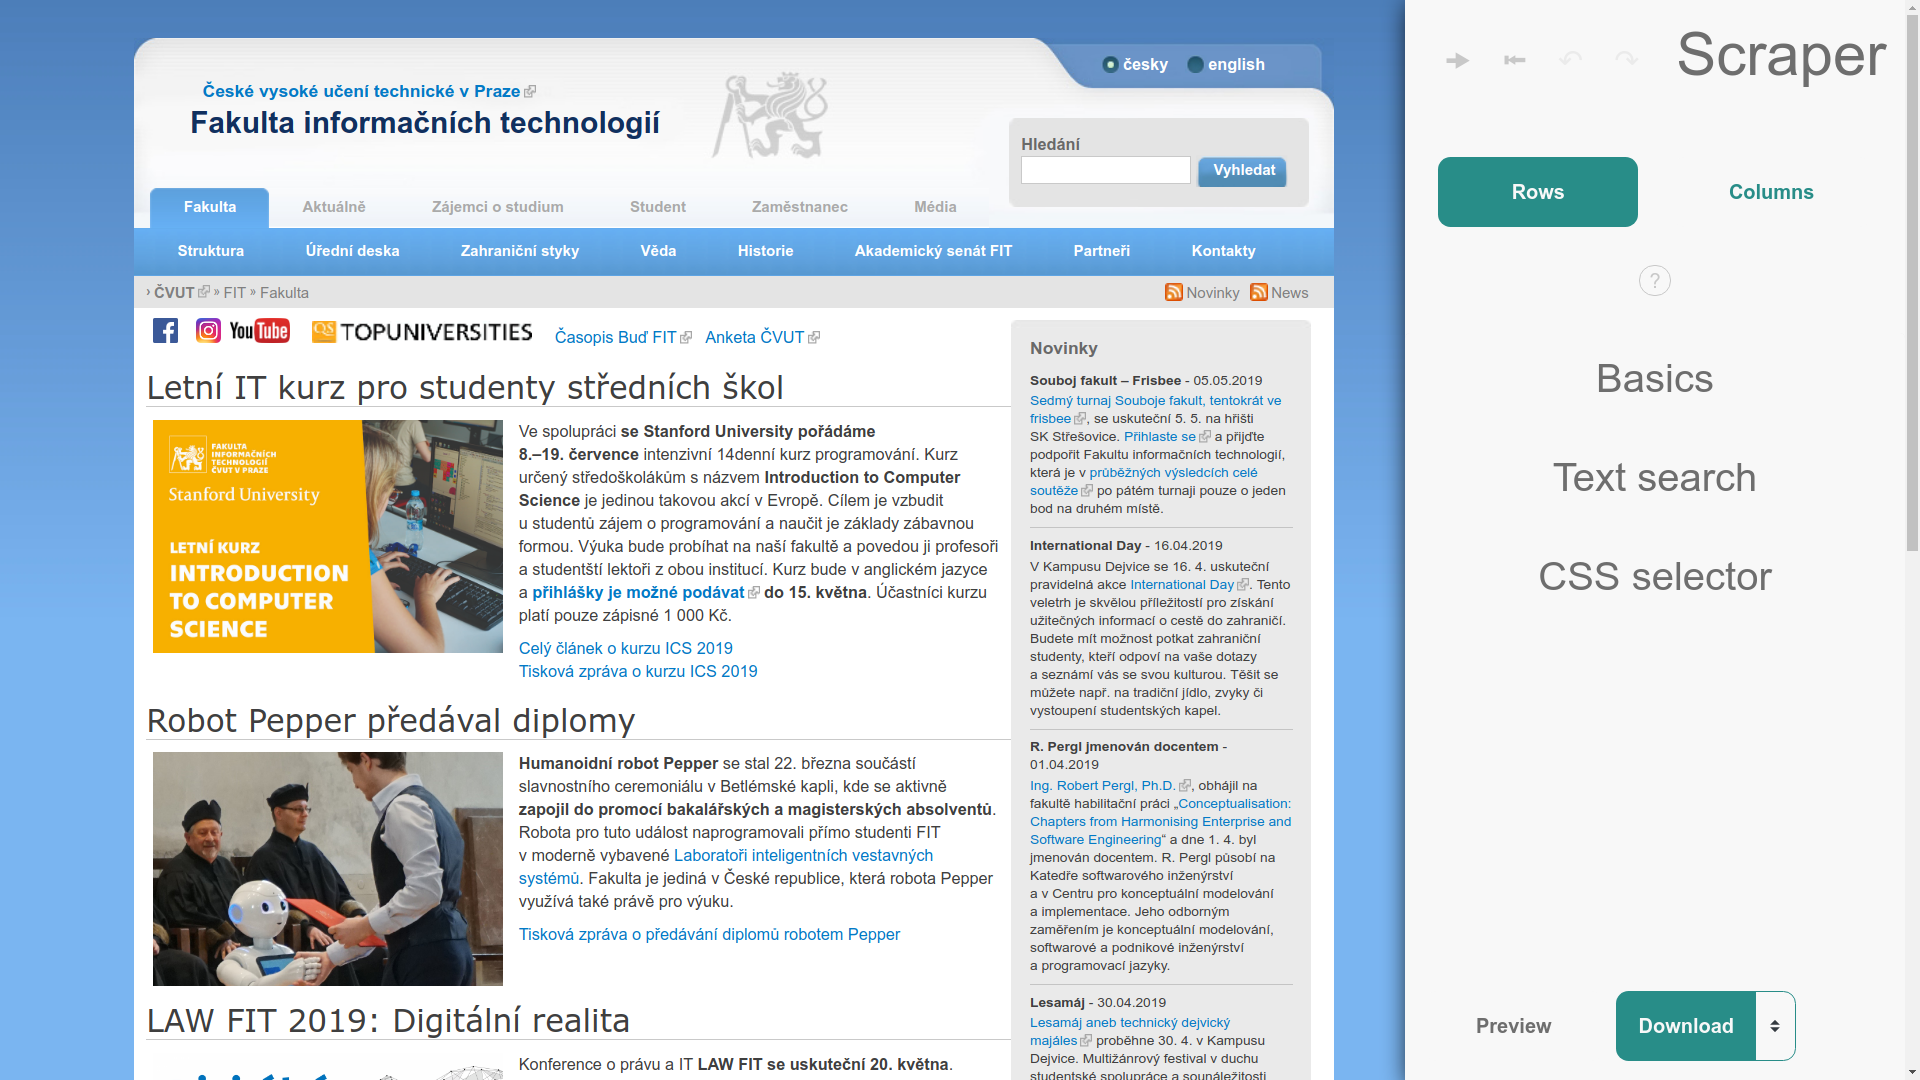
\includegraphics[width=\linewidth]{images/Scraper_control_panel.png}
		\caption{Ovládací panel aplikace}
		\label{fig:scraper_control_panel}
	\end{figure}

	Jak jsme si řekli v úvodu, výsledná data budou ve formě tabulky, tedy musíme vybrat, které elementy na stránce budou reprezentovat řádky výsledné tabulky a které budou reprezentovat sloupce, viz Obrázek \ref{fig:scraper_rows_cols}. K tomu slouží dvě velká tlačítka \textsf{Rows} a \textsf{Columns}, kterými se přepíná výběr právě mezi řádky a sloupci. Doporučený postup je nejdřív vybrat řádky\footnote{To budou nejčastěji různé \uv{kontejnery}, které sdružují data jedné entity dohromady -- jako příklad lze uvést kartu produktu v přehledu produktů e-shopu.} a poté uvnitř těchto větších elementů vybírat sloupce\footnote{To může být například cena nebo jméno daného produktu.}.
	\begin{figure}
		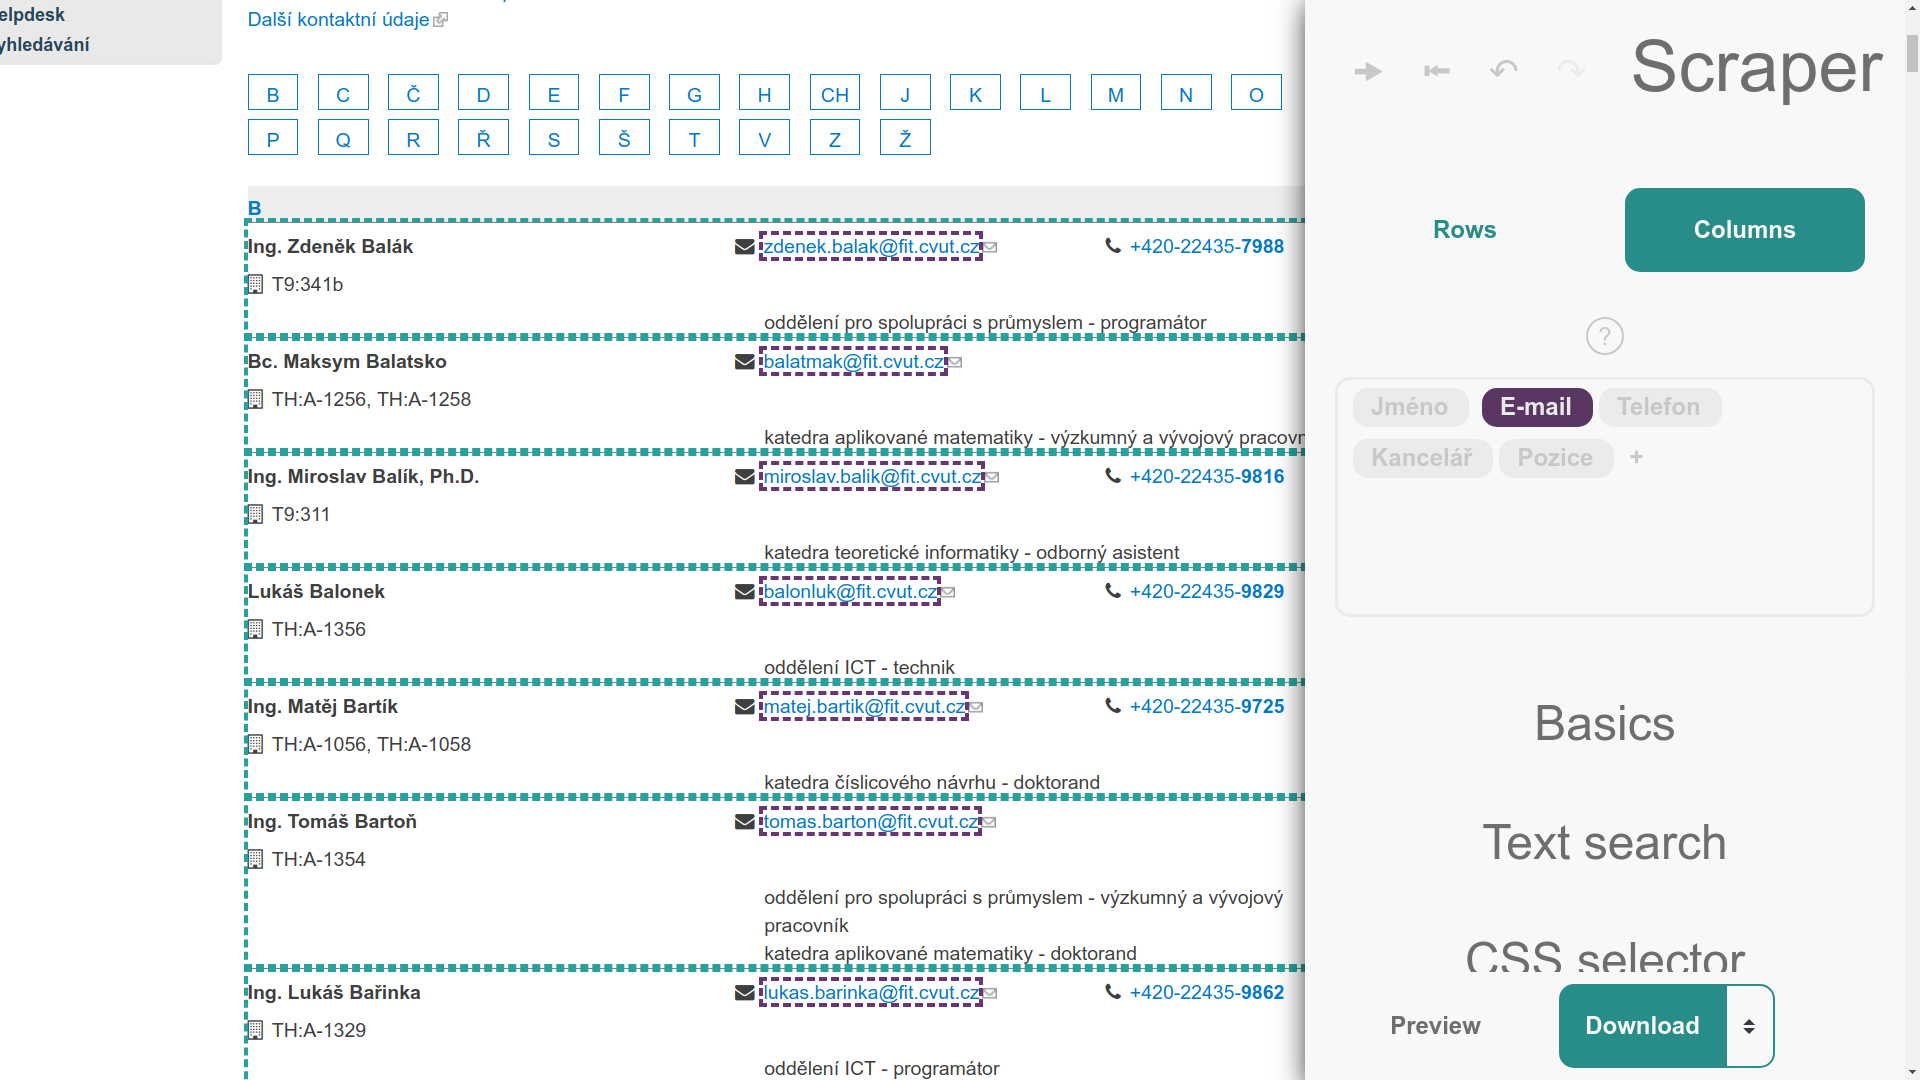
\includegraphics[width=\linewidth]{images/Scraper_rows_cols.png}
		\caption{Výběr řádků (tyrkysově) a sloupců (vínově)}
		\label{fig:scraper_rows_cols}
	\end{figure}
	
	Dle zadání v kapitole Návrh, sekce Specifikace požadavků, probíhá selekce třemi způsoby -- ruční označování prvků, hledání na základě textové shody a výběr pomocí CSS selektorů. Tyto tři druhy výběru jsou stejné jak pro výběr řádků, tak pro výběr sloupců. Jakýkoli výběr lze vzít zpět nebo následně provést znovu pomocí tlačítek \textsf{Undo} a \textsf{Redo} v horní části nástroje. Následuje popis každého ze způsobů výběru:
	\begin{description}
		\item[Ruční označování] se nachází na kartě \textsf{Basics} a probíhá jednoduše klikáním myši na požadované elementy. Pokud uživatel při vybírání podrží klávesu \textsf{Ctrl/control}, aplikace se pokusí vybrat všechny podobné prvky na základě předchozího kliknutí. Kliknutím na již označený element se výběr zruší.
		
		Největší část výběrů bude představovat právě tento způsob.
		\item [Textová shoda] se nalézá na kartě \textsf{Text search}, která se skládá ze tří samostatných formulářů. Uživatel má možnost vybrat všechny elementy na stránce, jejichž text buď:
		\begin{enumerate}[a)]
			\item začíná daným výrazem,
			\item končí daným výrazem,
			\item obsahuje daný výraz nebo se mu přímo rovná.
		\end{enumerate}
		Tento způsob se osvědčí například v případě, kdy chceme vybrat všechny e-mailové adresy na stránce -- stačí hledat prvky, které obsahují zavináč.
		\item [CSS selektory] najdeme na kartě s názvem \textsf{CSS selectors} a jedná se o jednoduché textové pole, které přijímá libovolný CSS selektor. Můžeme tedy pomocí něj vybírat na základě HTML tagů (\textsf{jmenoTagu}), tříd (\textsf{.jmenoTridy}), atributů (\textsf{[atribut=hodnota]}), různé následnosti (\textsf{otec $>$ syn $+$ naslednik}) a zkrátka vše, co CSS selektory umí, viz \href{https://www.w3schools.com/cssref/css_selectors.asp}{přehled selektorů}.
		
		Toto je jistě nejsilnější z uvedených způsobů, jelikož s ním jde vybrat libovolná skupina prvků, avšak předpokládá alespoň základní znalost HTML, CSS a především struktury stránky. Je tedy spíš pro pokročilejší uživatele.
	\end{description}
	\begin{figure}[h]
		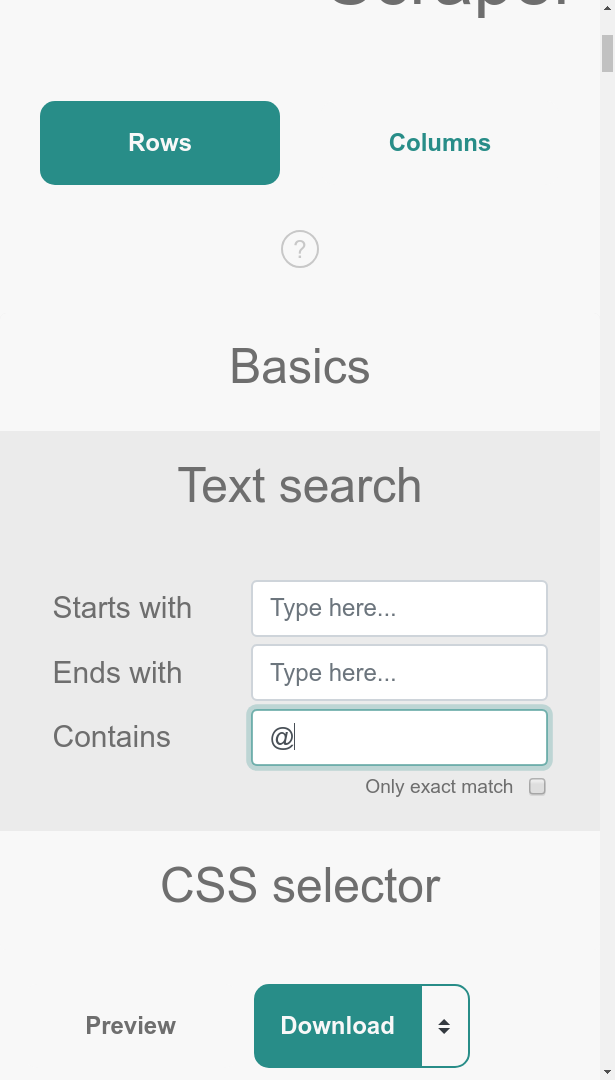
\includegraphics[width=\linewidth]{images/Scraper_text_search.png}
		\caption{Výběr na základě textové shody}
		\label{fig:scraper_text_search}
	\end{figure}

	Může se stát, že požadovaný element nejde označit ručně. Pro tyto případy je každý vybraný prvek opatřen čtveřicí tlačítek, která se objeví, pokud uživatel najede kurzorem na daný element, viz Obrázek \ref{fig:scraper_dom_navigation}. Tlačítko \textsf{$+$} posune označení na prvního syna, \textsf{$-$} na otce prvku, \textsf{$\leftarrow$} na předchozího sourozence a tlačítko \textsf{$\rightarrow$} na následujícího sourozence. Tímto způsobem může uživatel traverzovat napříč celým DOMem a vybrat tak libovolný prvek.
	\begin{figure}[h]
		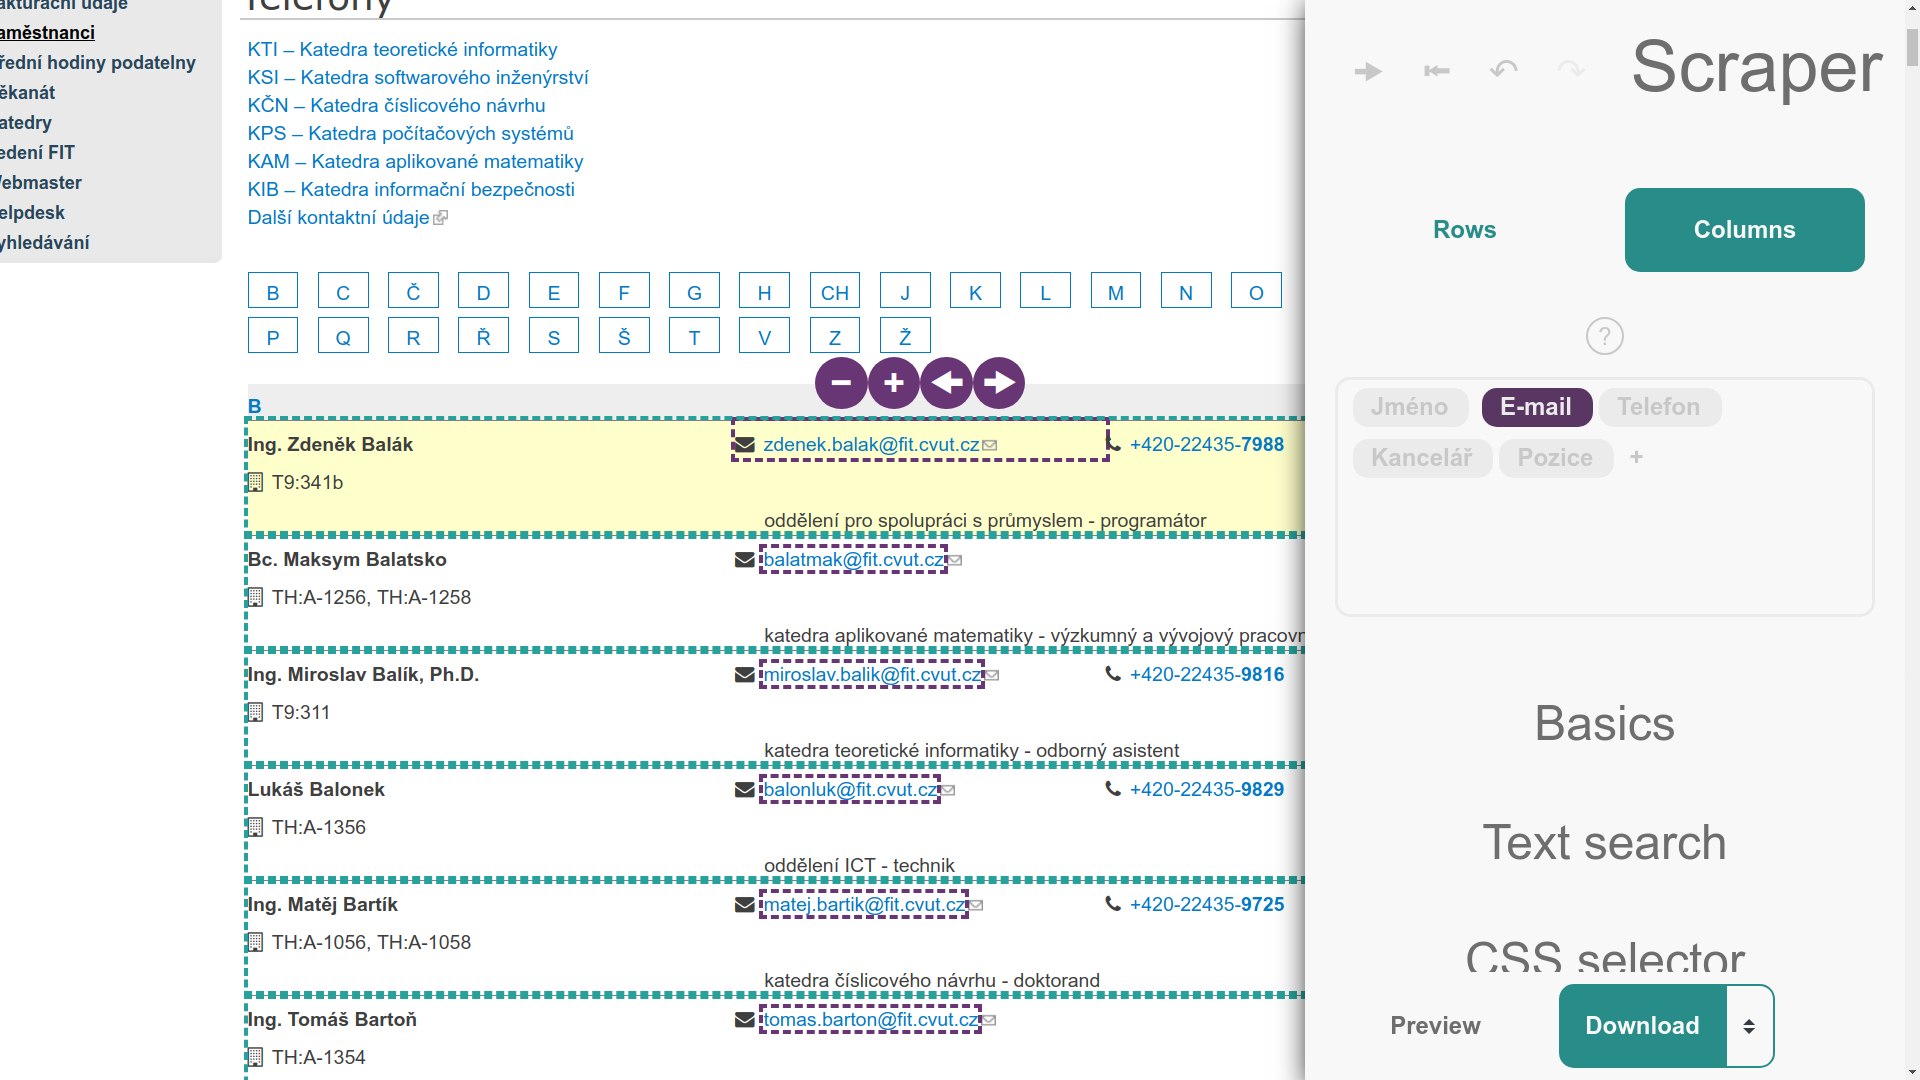
\includegraphics[width=\linewidth]{images/Scraper_dom_navigation.png}
		\caption{Navigace výběru napříč dokumentem}
		\label{fig:scraper_dom_navigation}
	\end{figure}

	Poté, co jsme s výběrem hotovi, je možné data prohlídnout v tzv. \textit{Preview módu}. Zobrazí se tabulka obsahující námi zadané řádky a sloupce\footnote{Nutno podotknout, že prvky označené jako sloupce, které se \emph{nenacházejí} uvnitř prvku označeného jako řádek, nebudou zahrnuty do výsledku.}. V tuto chvíli je možné zkontrolovat veškerá extrahovaná data a případně vyřadit ta, která nevyhovují našim potřebám pomocí křížku na levé straně každého řádku (ten se objeví až po najetí kurzorem na daný řádek), viz Obrázek \ref{fig:scraper_preview_mode}. Vyřazení záznamu způsobí zrušení výběru elementů, které obsahují příslušná data.
	\begin{figure}[h]
		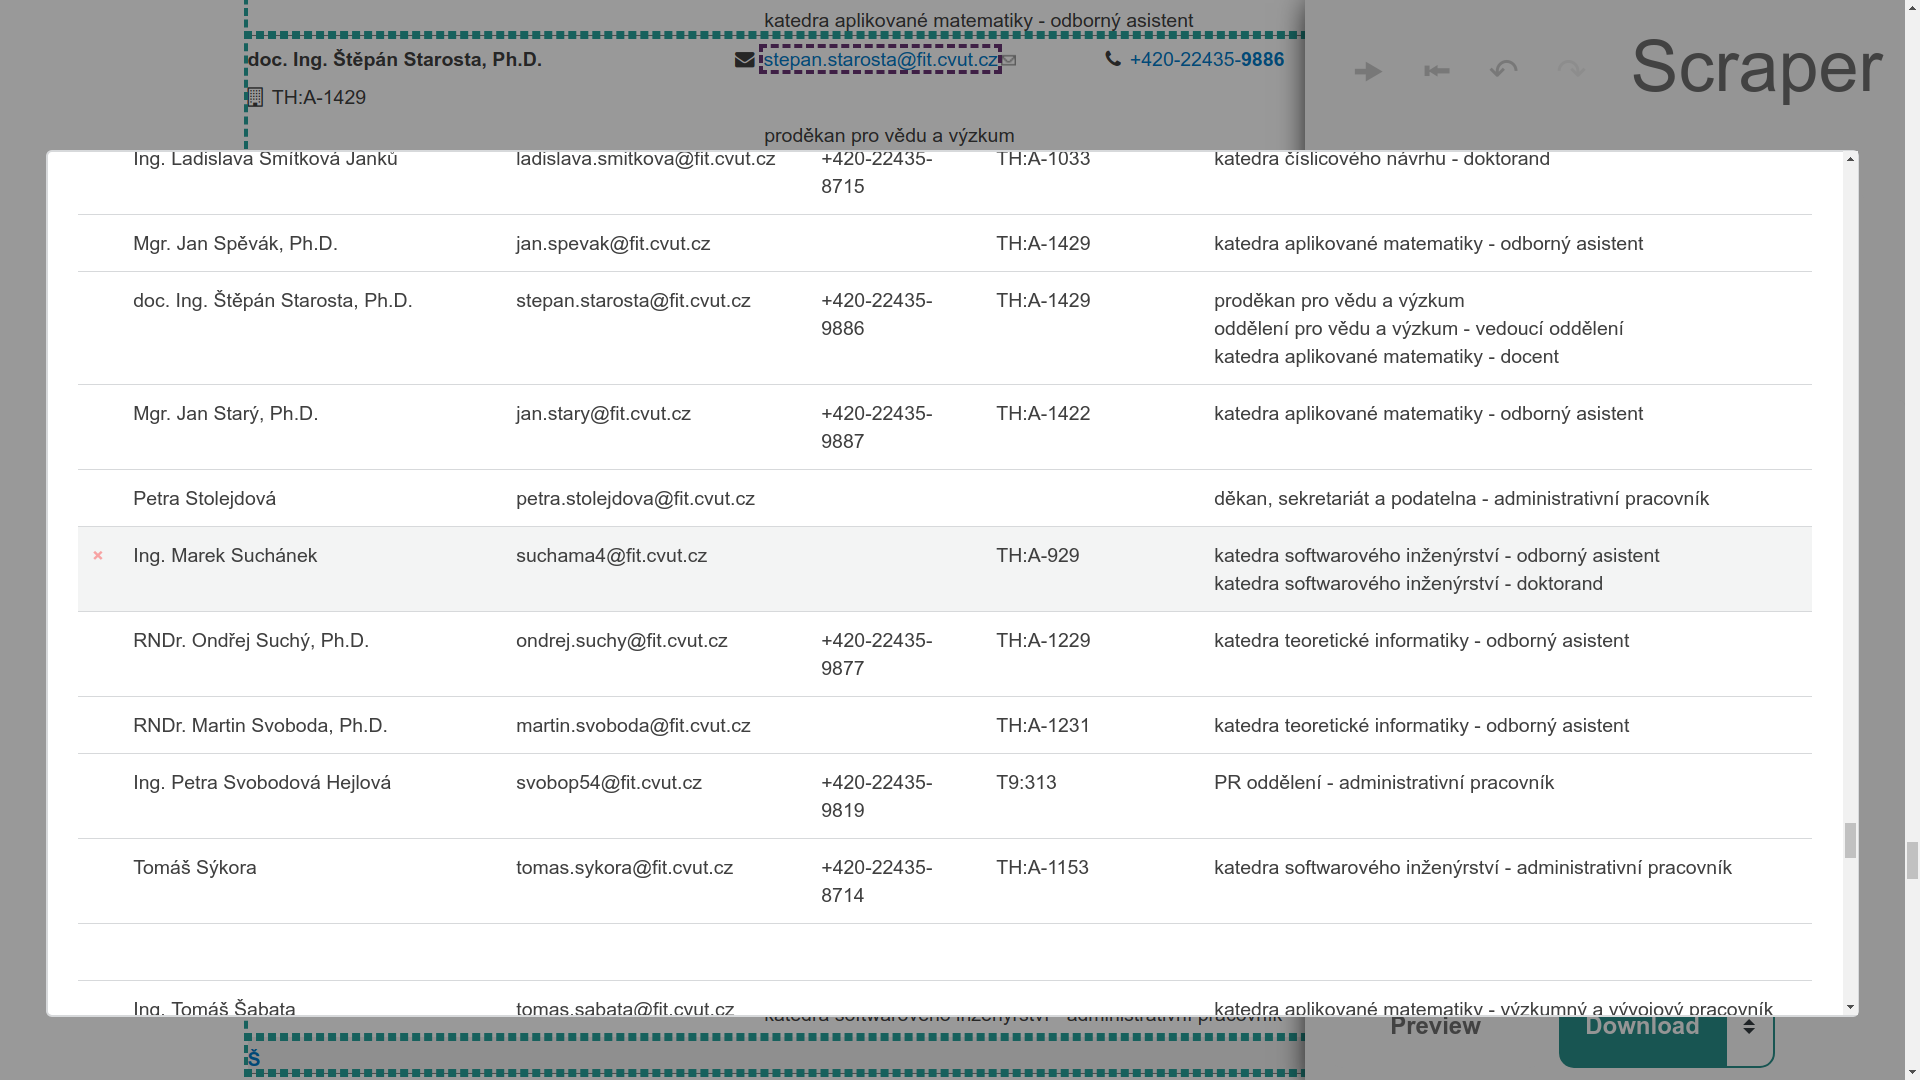
\includegraphics[width=\linewidth]{images/Scraper_preview_mode.png}
		\caption{Tabulka obsahující náhled extrahovaných dat}
		\label{fig:scraper_preview_mode}
	\end{figure}

	Na závěr stačí pomocí rozbalovacího výběru zvolit formát, do kterého chceme data exportovat (zatím je na výběr CSV a JSON) a kliknout na tlačítko \textsf{Download}.
	
	\section{Implementace zvoleného řešení}
	\subsection{Inicializace a spuštění}
	Jak již bylo řečeno v úvodu této kapitoly, použité řešení spočívá ve vložení ovládacího panelu do libovolné stránky. To umožňuje právě komponenta \hyperref[def:content_script]{content script}, jež byla zmíněna výše. Základní běh aplikace vypadá následovně:
	\begin{enumerate}
		\item Po instalaci rozšíření do prohlížeče Google Chrome (a každém jeho spuštění) je vykonán kód, který je obsažen v background scriptu. Zde se nachází pouze obsluha vyzývající content script k zobrazení nebo schování ovládacího panelu.
		\item Když je rozšíření aktivní, do \emph{každé} načtené stránky je vložen content script, jenž poslouchá zprávy od background scriptu.
		\item Kliknutím na ikonu rozšíření v hlavním panelu nástrojů prohlížeče je vyvolána událost, na kterou reaguje background script -- aktivnímu oknu/záložce zašle zprávu, aby byl otevřen ovládací panel. 
		\item Tu odchytí content script, který na dané stránce poslouchá a vloží do těla stránky nový iframe, do něhož načte HTML dokument, který představuje samotný ovládací panel. Při další žádostech je iframe pouze skryt/zobrazen.
		\item Vhodným nastavením příslušných CSS vlastností je iframe umístěn na boční straně prohlížené stránky a nabývá formy ovládacího panelu. 
	\end{enumerate}
	Obrázek \ref{fig:scraper_control_panel} ilustruje, jak ovládací panel vypadá po vložení do stránky.

	\subsection{Výběr dat}
	\dots
	
	\subsection{Komunikace mezi komponentami}
	\dots
	
	\subsection{Extrakce dat}
	\dots
	
	\subsection{Ostatní}
	\dots
	
	% ================================================================================================
	
	\chapter{Testování}
	
	% ================================================================================================
	
	\begin{conclusion}
		%sem napište závěr Vaší práce
	\end{conclusion}
	
	\bibliographystyle{csn690}
	
	\begin{thebibliography}{9}
		\bibitem{parsehub}
		PARSEHUB. \textit{ParseHub. Version 54.0.1} [software]. 2015 [cit. 13. 4. 2019]. Dostupné z: \url{https://www.parsehub.com/quickstart}.
		
		\bibitem{octoparse}
		OCTOPUS DATA INC. \textit{Octoparse. Version 7.1.2} [software]. 2018 [cit. 13. 4. 2019]. Dostupné z: \url{https://www.octoparse.com/download}.
		
		\bibitem{webscraper}
		WEBSCRAPER. \textit{WebScraper. Version 0.3.8.9} [software]. 2016 [cit. 13. 4. 2019]. Dostupné z: \url{https://chrome.google.com/webstore/detail/web-scraper/jnhgnonknehpejjnehehllkliplmbmhn}.
		
		\bibitem{dexio}
		DEXI APS. \textit{Dexi.io} [software] [cit. 13. 4. 2019]. Dostupné z: \url{https://app.dexi.io/}.
		
		\bibitem{data_scraper}
		SOFTWARE INNOVATION LAB LLC. \textit{Data scraper. Version 3.299.84} [software]. 2015 [cit. 13. 4. 2019]. Dostupné z: \url{https://chrome.google.com/webstore/detail/data-scraper-easy-web-scr/nndknepjnldbdbepjfgmncbggmopgden}.
		
	\end{thebibliography}

	\appendix
	
\end{document}
